\documentclass[11pt]{standalone}

\usepackage{amsmath}
\usepackage{ifthen}
\usepackage{tikz} 
\usetikzlibrary{shapes.misc}
\usetikzlibrary{arrows,arrows.meta}
\usetikzlibrary{calc,intersections, patterns, math}

\definecolor{pfeil}{RGB}{168,167,167}
\definecolor{petrol}{RGB}{0, 118, 136}
\definecolor{darkgoldenrod}{RGB}{184, 134, 11}
\colorlet{petrol-lighter}{petrol!40}
\colorlet{darkgoldenrod-lighter}{darkgoldenrod!40}

\renewcommand{\d}{\text{\,d}}

\begin{document}

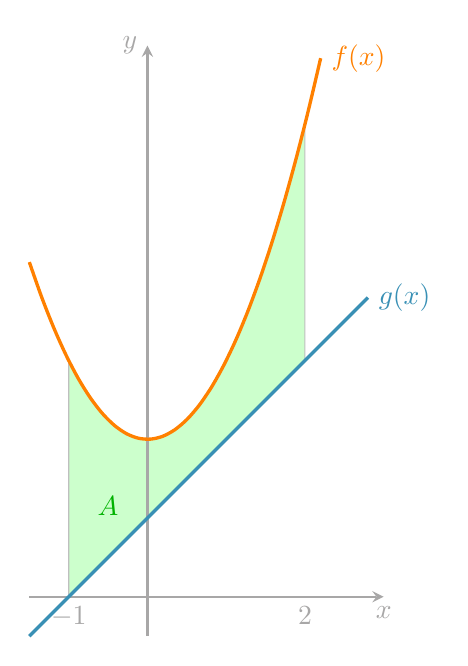
\begin{tikzpicture}[pfeil]

	% \draw[thick, fill=petrol!20, draw=petrol-lighter, rounded corners=2ex, opacity=0.5] (0,0) rectangle ++ (1.5,3.5);
	% \draw[thick, fill=darkgoldenrod!20, draw=darkgoldenrod-lighter, rounded corners=2ex, opacity=0.5] (5,0) rectangle ++ (1.5,3.5);

	% \draw[thick, -stealth] (-4.5,0) -- (4.5,0) node[below]{$\scriptstyle x$};
	% \draw[thick, -stealth] (0,-2.5) -- (0,2.5) node[left]{$\scriptstyle y$};


	\path[thin, draw=lightgray, fill=green!20] plot[domain=-1:2](\x,{\x*\x+2}) -- plot[domain=2:-1] (\x,{\x+1}) --cycle;
	\draw[thick,-stealth] (-1.5,0) -- (3,0) node[below]{$x$};
	\draw[thick,-stealth] (0,-0.5) -- (0,7) node[left]{$y$};
	\node[below] at (-1,0) {$-1$};
	\node[below] at (2,0) {$2$};
	\node[green!70!black] at (-0.5,1.15) {$A$};
	\draw[domain=-1.5:2.2, very thick, orange, smooth] plot(\x,{\x*\x+2}) node[right] {$f(x)$};
	\draw[domain=-1.5:2.8, very thick, cyan!70!black, smooth] plot(\x,{\x+1}) node[right] {$g(x)$};

\end{tikzpicture}

\end{document}
